\section{Results}
\label{sec:chap_slam_results}

In this section, we evaluate the performance of the place recognition algorithm on our three datasets. We then compare the results between the unstructured and structured environments as well as between the SICK and the Velodyne acquisitions. 

\subsection{Performance Evaluation}
\label{ssec:chap_slam_performance_evaluation}

The evaluation of the place recognition performance is based on two crucial task: the identification of real world places and the identification of scans originating from the same place. We will first discuss the method used to perform these tasks and present the associated data. Afterwards, we will conduct the performance evaluation itself.

\subsubsection{Identification of Real World Places}
The notion of a place can be variable, but the closer two points of the space are to each other, the more likely they are to be considered in the same place. Therefore, we use the real world physical distance between two acquisitions as an indicator of the likelihood that they represent the same place. \todo{Talk about the binary label here or not ?}

We will now discuss the method used to determine the distance between scans. We first used the robot odometry as a rough approximation of the relative pose between two subsequent scans. In order to reduce the pose estimation error, we then used the \gls*{icp} algorithm to align the two point clouds and adjust the odometry accordingly. These steps were performed sequentially for all scans of the first loop. This technique can not be independently repeated for the second loop, because the difference in error accumulation would cause a discrepancy between the resulting path of the two loops. To address this problem, the \gls*{icp} odometry adjustment of the second loop was performed relative to the first loop. To do this, we first align the first scan of the second loop relative to the first scan of the first loop using \gls*{icp}. Thereafter, each scan of the second loop was adjusted with respect to the scan of the first loop theoretically being closest, considering the last corrected pose and the movement of the robot. Figure~\ref{fig:chap_slam_results_paths} illustrates the resulting paths as well as the position of each scans for our three datasets. Note that this is a 2D representation for which the vertical component was ignored. This figure shows the absence of discrepancy between the 2 loops of one dataset.

With the corrected odometry it is possible to easily obtain the distance between two scans. To do this, one can simply calculate the norm of the difference in position between the two scans. On the other hand, given the accumulated odometry error, the relative position between the last scan of a loop $L_i$ and the first scan of a loop $L_j$ (including $i=j$) can be significant. The relative error generally also increases over time (each move to a new acquisition). To reduce the impact of these problems, we used \gls*{icp} to determine the relative pose for all pair \textit{(first scan, last scan)}. With these relative poses, it was possible to create the reverse sequential path between two scans. Finally, we use the path for which the scans are closest in terms of acquisition numbers (sequential or reverse) for the final calculation of the distance.

Note that all alignments have been visually inspected to ensure that \gls*{icp} had indeed converged to a valid solution. When this was not the case, the odometry provided by the robot was manually adjusted to enable this convergence. The second line of Figure~\ref{fig:chap_slam_results} show the resulting distances matrices for all pair of scans for each of our 3 datasets. Note that a distance function is by definition symmetrical, therefore producing a symmetrical matrix. The values on the main diagonal represent the distance between a scan and itself and are therefore null. A secondary diagonal of low values is produced by the small distances between the scans of the first and the second loop. Finally, because we tried to stop the loop acquisitions approximately at the starting point, we observe small values at those junction points.


\subsubsection{Identification of Scan Places}
For our experiments, we used a \textit{C++} implementation of the place recognition algorithm. Thanks to Bastian Steder who provided us the source code. The resulting software allowed us to obtain a score (between 0 and 1) for each pair of scan in the database. 

\begin{itemize}
    \item Element 2: Le Code utiliser pour determiner le score entre chaque pair de scan est une implementation c++ de l'algo presente a la section X, qui nous a ete fourni par B.S. Le score se trouve en 0 et 1 (0 mauvais et 1 super bon)
    \item La matrice n'est pas parfaitement symetrique parce que f(a,b) != f(b,a), mais difference negligeable, nous utiliserons uniquement la partie inferieure gauche excluant la diagonale.
    \item The dark areas that are not close to the main diagonal mark loop closures.
\end{itemize}

\subsubsection{Evaluation}
\label{ssec:chap_slam_results_evaluation}

\begin{itemize}
    \item Even though it is interesting to analyse the performance using continous values, the place recognition task most often require a binary output (either recognized or not)
    \item Expliquer qu'il est important de n'avoir aucun FP car cause des fausses loop closures
    \item Introduire les thresholds uniquement pour le graphique de recall... Ces deux mesures sont continues et doivent etre binairiser afin de poser une decision finale, TP,FN,TN,FP
\end{itemize}


\begin{figure}[H]
    \centering
    \subfloat[]{\label{fig:building_paths_plot}}{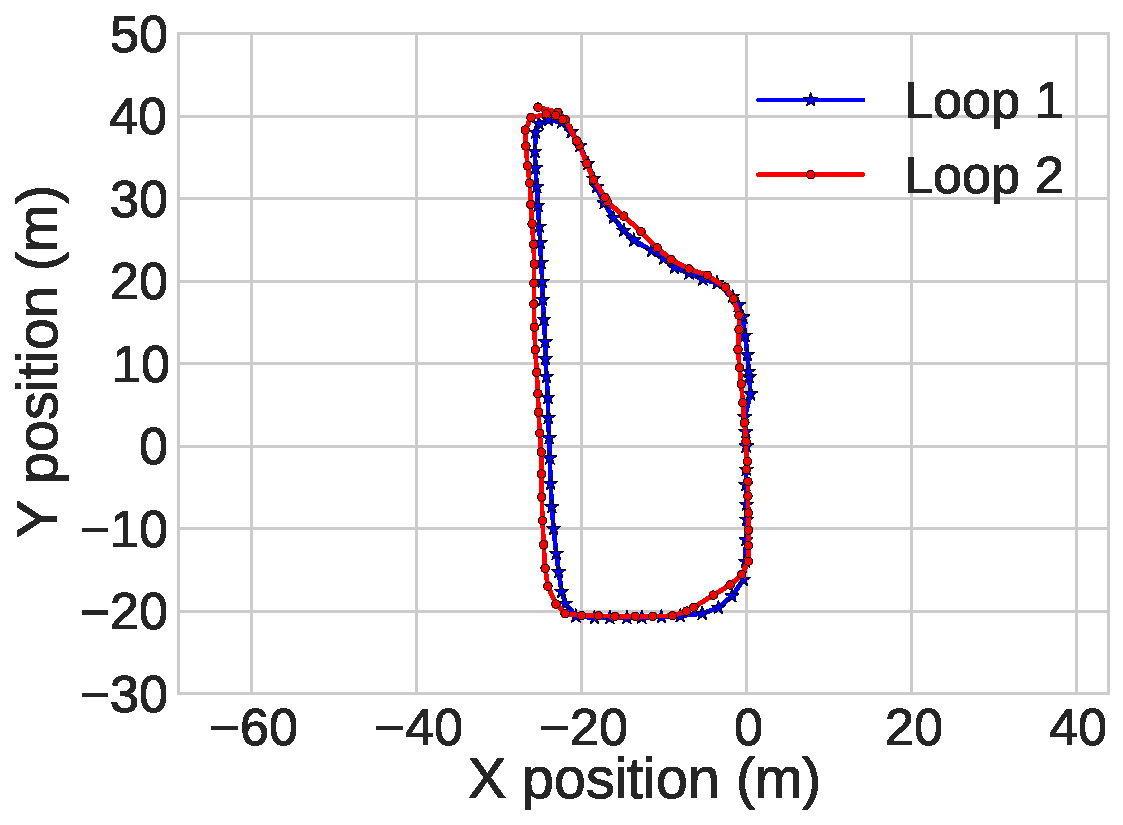
\includegraphics[width=0.31\linewidth]{img/chap_slam/building_paths.pdf}}
    \subfloat[]{\label{fig:forest_paths_plot}}{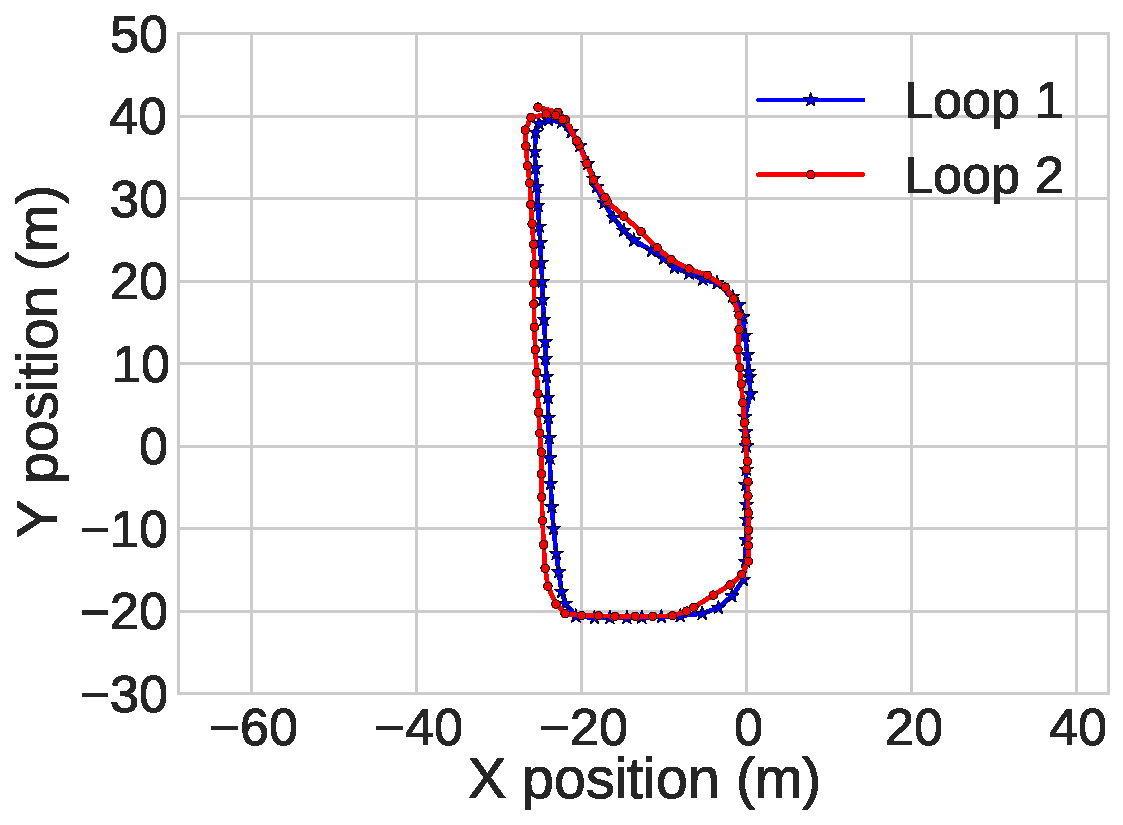
\includegraphics[width=0.31\linewidth]{img/chap_slam/building_paths.pdf}}
    \subfloat[]{\label{fig:velodyne_paths_plot}}{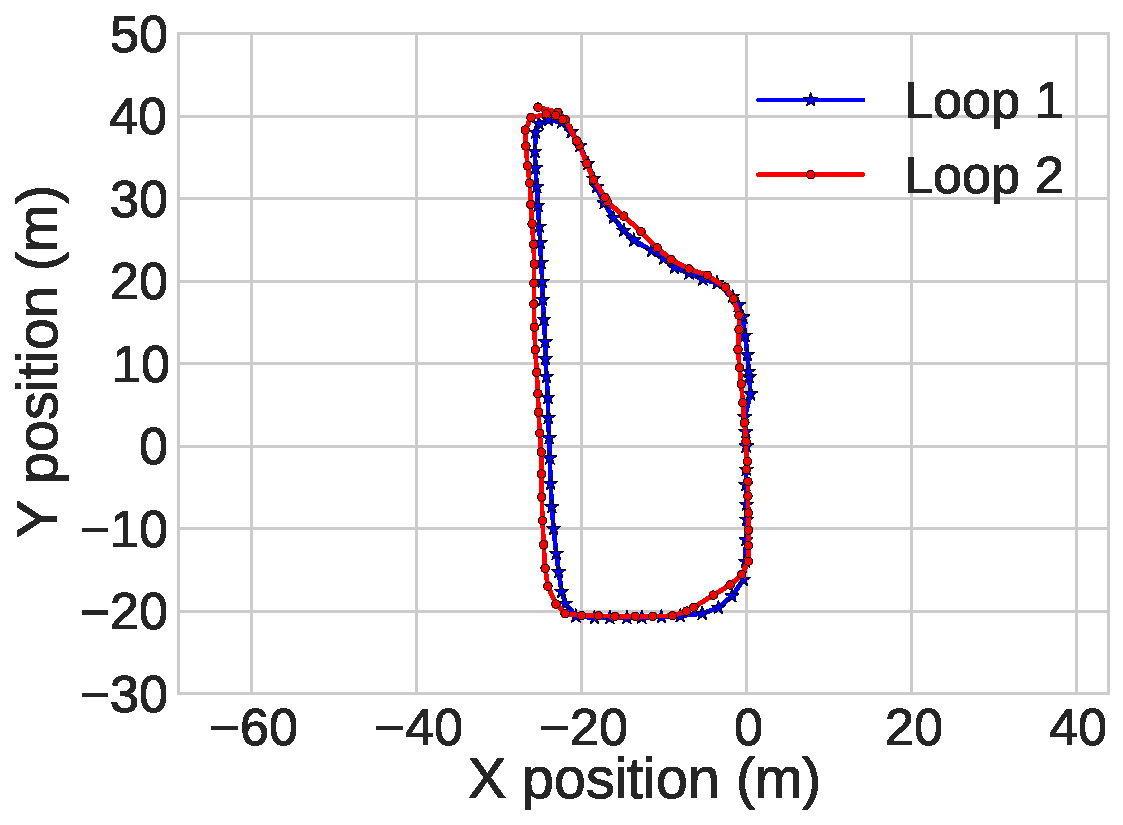
\includegraphics[width=0.31\linewidth]{img/chap_slam/building_paths.pdf}}
    \caption[todo]{\todo{Hum... quite small...}}
    \label{fig:chap_slam_results_paths}
\end{figure}

\begin{figure}[H]
    \centering
    \subfloat[]{\label{fig:building_scores_matrix}}{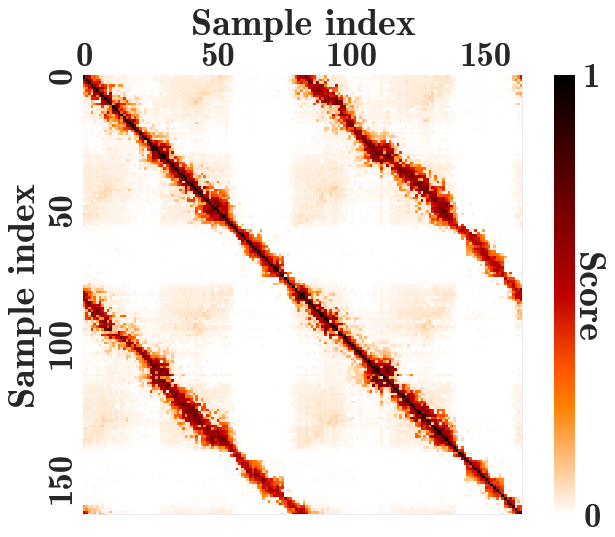
\includegraphics[width=0.31\linewidth]{img/chap_slam/building_scores_matrix.png}}
    \subfloat[]{\label{fig:forest_scores_matrix}}{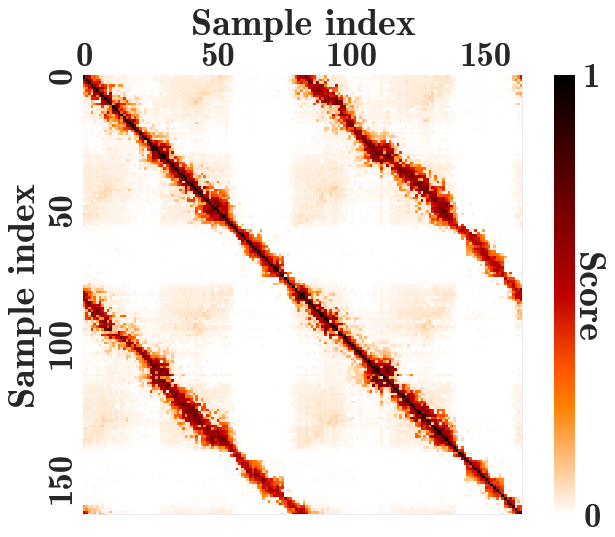
\includegraphics[width=0.31\linewidth]{img/chap_slam/building_scores_matrix.png}}
    \subfloat[]{\label{fig:velodyne_scores_matrix}}{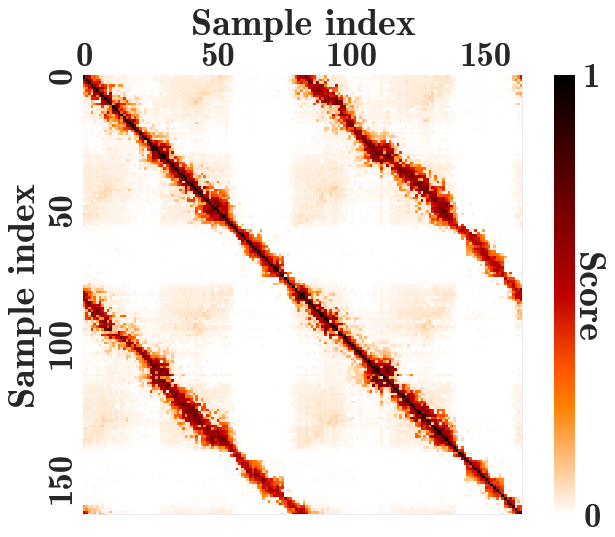
\includegraphics[width=0.31\linewidth]{img/chap_slam/building_scores_matrix.png}} \\

    \subfloat[]{\label{fig:building_distances_matrix}}{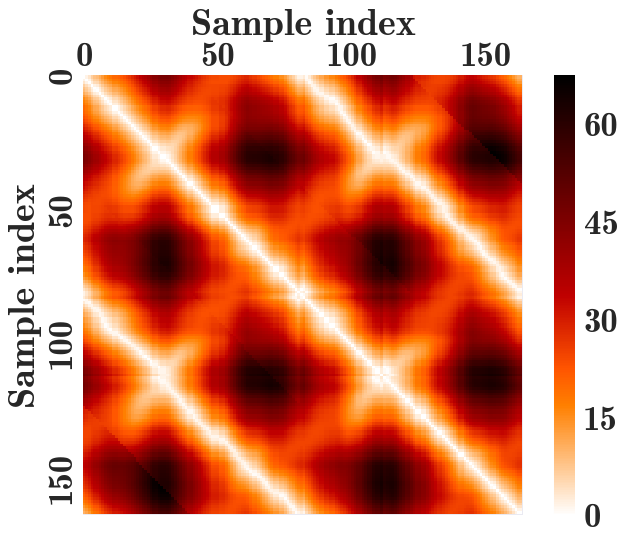
\includegraphics[width=0.31\linewidth]{img/chap_slam/building_distances_matrix.png}}
    \subfloat[]{\label{fig:forest_distances_matrix}}{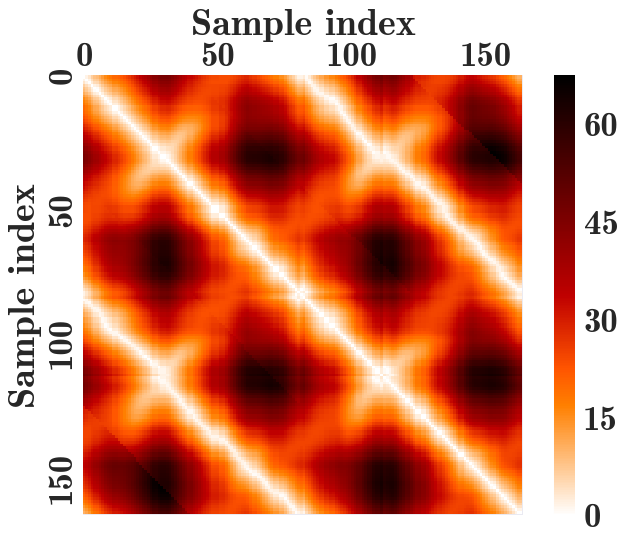
\includegraphics[width=0.31\linewidth]{img/chap_slam/building_distances_matrix.png}}
    \subfloat[]{\label{fig:velodyne_distances_matrix}}{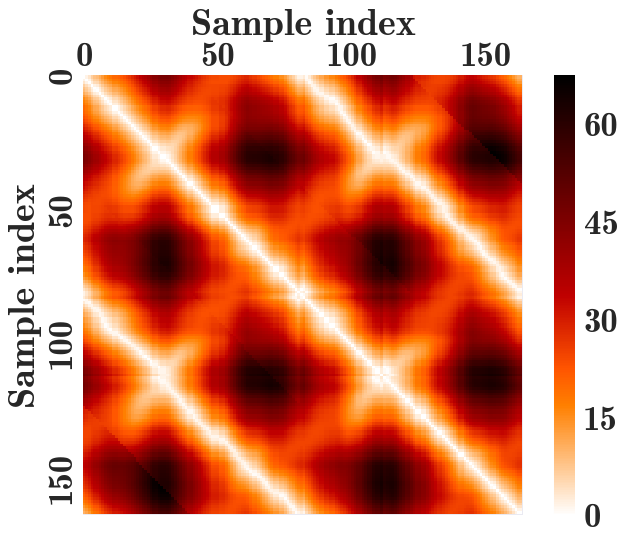
\includegraphics[width=0.31\linewidth]{img/chap_slam/building_distances_matrix.png}} \\

    \subfloat[]{\label{fig:building_distances_scores_plot}}{\includegraphics[width=0.31\linewidth]{img/chap_slam/building_distances_scores_plot.pdf}}
    \subfloat[]{\label{fig:forest_distances_scores_plot}}{\includegraphics[width=0.31\linewidth]{img/chap_slam/building_distances_scores_plot.pdf}}
    \subfloat[]{\label{fig:velodyne_distances_scores_plot}}{\includegraphics[width=0.31\linewidth]{img/chap_slam/building_distances_scores_plot.pdf}}

    \subfloat[]{\label{fig:building_recall_plot}}{\includegraphics[width=0.31\linewidth]{img/chap_slam/building_recall_plot.pdf}}
    \subfloat[]{\label{fig:forest_recall_plot}}{\includegraphics[width=0.31\linewidth]{img/chap_slam/building_recall_plot.pdf}}
    \subfloat[]{\label{fig:velodyne_recall_plot}}{\includegraphics[width=0.31\linewidth]{img/chap_slam/building_recall_plot.pdf}}
    \caption[todo]{\protect\subref{fig:result_matrix_structured} is the confusion matrix for both loops of the structured dataset (XX scans) and \protect\subref{fig:result_curve_structured} is the recall curve. \protect\subref{fig:result_matrix_forest} and \protect\subref{fig:result_curve_forest} are the corresponding matrix and recall curve for the unstructured dataset and \protect\subref{fig:result_matrix_forest} and \protect\subref{fig:result_curve_forest} are for the unstructured dataset using the velodyne.}
    \label{fig:chap_slam_results}
\end{figure}

%\begin{figure}[htpb]
    %\centering
    %
\includegraphics[width=0.2\linewidth]{img/todo.jpg}
    %\caption[todo]{Nice to have: matched keypoints (something like an histogram of dist, height or avg dist per scan)}
    %\label{fig:match_avg_dist}
%\end{figure}


\subsection{Comparative Analysis}
\label{ssec:chap_slam_comparative_analysis}

\subsection{Structured and Unstructured Environments}
\label{ssec:chap_slam_struct_vs_forest}
\begin{itemize}
    \item Because distance is smaller on avg in the forest, cause parallax
    \item Also more occlusion, but this also why the env. is complex. As said earlier range img kind of deal with it.
\end{itemize}

\subsection{SICK and Velodyne \gls*{lidar}s}
\label{ssec:chap_slam_sick_vs_velodyne}
